\documentclass[12pt, aspectratio=169, mathserif]{beamer}
\usepackage[utf8]{inputenc}
\usepackage{amstext}
\usepackage{amsmath}
\usepackage{graphicx}
\usepackage{amsfonts}
\usepackage{algorithm, algorithmic}
\floatname{algorithm}{Procedure}
\renewcommand{\algorithmicrequire}{\textbf{Input:}}
\renewcommand{\algorithmicensure}{\textbf{Output:}}
\title[MABP for the Optimal Design of Clinical Trials]{Review: Multi-armed Bandit Models for the Optimal Design of Clinical Trials: Benefits and Challenges}
\author[Ken Tanaka]{Ken Tanaka Hernández}
\institute[ICTP]{The Abdus Salam International Centre for Theoretical Physics\\\color{white}.\color{black}\\Project for Reinforcement Learning:\\Prof. Antonio Celani}
\logo{
\includegraphics[height=1.3cm]{../../logo.jpeg}}
\setbeamertemplate{navigation symbols}{}
\usetheme{Madrid}
\begin{document}
  \begin{frame}
    \titlepage
  \end{frame}
  \begin{frame}[t]
    \frametitle{Introduction}
    \framesubtitle{Multi-armed Bandit}
    \begin{columns}
      \begin{column}{0.4\textwidth}
        $p(s'|s,a)=\mathbb{I}(s'= s)$\\
        $\text{Ber}(\rho), \rho\in(0,1)$\\
        $p(\rho|s=(q)_j, a = i) = q_i^\rho(1 - q_i)^{1-\rho}/A$
      \end{column}
      \begin{column}{0.6\textwidth}
        $s=(q_1,q_2) \rightarrow b(s) = P(q_1, q_2)$\\
        $p(\rho|b(s), a) = \int dsb(s)p(r|s, a)$\\
        $p(\rho|b(q_1, q_2), 1) = \int dq_1dq_2P(q_1, q_2)q_1^\rho(1-q_1)^{1-\rho}$\\
        $b'(q|r) = {q^r (1-q)^{(1-r)} \,\,\, b(q)} \,\,\,\, / {\int dq b(q)}$\\
        $V_\pi(b) = \mathbb{E}_\pi\bigg[ \sum_{t=0}^\infty \gamma^t\,r_t \Big| b_0 = b \bigg]$
        $V^*(b) = \max_{a\in\{1,2\}} \sum_{b'} p(b'|b,a)\big[ r(b',b) + \gamma V^*(b') \big]$
      \end{column}
    \end{columns}
  \end{frame}
  \begin{frame}[t]
    \frametitle{Naive Algorithms}
    \framesubtitle{Explore Then Commit (ETC)}
    \begin{algorithm}[H]
      \begin{algorithmic}[1]
        \REQUIRE $m$
        \STATE $\forall t$
        \begin{equation*}
          A_t = \left\{\begin{matrix}
            (t\mod k), \text{if } t\leq mk;\\
            \text{argmax}_i\hat{\mu}_i(mk), t > mk
          \end{matrix}\right.
        \end{equation*}
      \end{algorithmic}
      \caption{Explore Then Commit (ETC)}
      \label{alg:seq}
    \end{algorithm}
  \end{frame}
  \begin{frame}
    \frametitle{Naive Algorithms}
    \framesubtitle{Explore Then Commit (ETC)}
    \begin{columns}
      \begin{column}{0.7\textwidth}
        \begin{equation*}
          R_n = \sum_{a \in \mathcal{A}}\Delta_a\mathbb{E}[T_a(n)]
        \end{equation*}
        \begin{equation*}
          R_n \leq m\sum_{i = 1}^k\Delta_i + (n -mk)\sum_{i = 1}^k\Delta_i\exp\left(-\frac{m\Delta_i^2}{4}\right)
        \end{equation*}
      \end{column}
      \begin{column}{0.3\textwidth}
        
\includegraphics[width=\textwidth]{Screenshot from 2023-07-12 13-50-37.png}
      \end{column}
    \end{columns}
  \end{frame}
  \begin{frame}[t]
    \vspace{-1cm}
    \begin{center}
      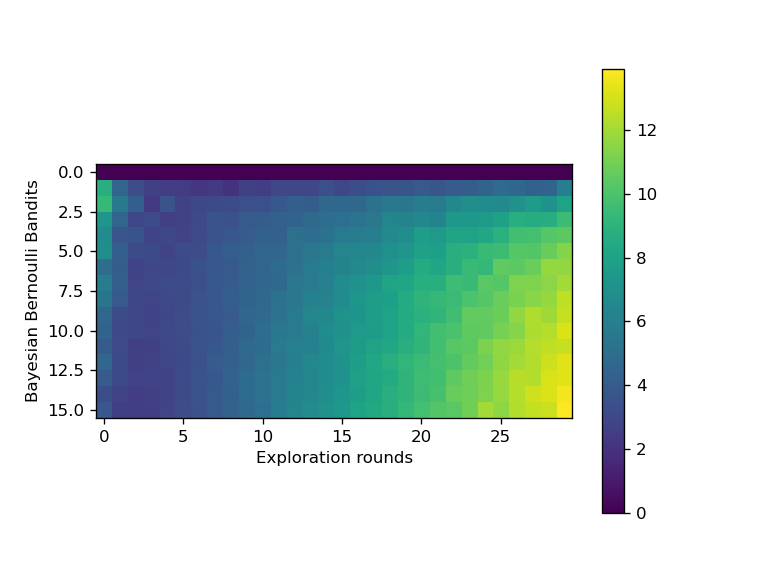
\includegraphics[height=1.1\textheight]{Figure 6.png}
    \end{center}
  \end{frame}
  \begin{frame}[t]
    \frametitle{Naive Algorithms}
    \framesubtitle{Explore Then Eliminate (ETE)}
    \begin{algorithm}[H]
      \begin{algorithmic}[1]
        \REQUIRE $k \text{ and } (m_l)_l$
        \STATE $A_1 = {1, \ldots, k}$
        \FOR{$l = 1,\ldots$}
          \STATE Choose each arm $i\in A_l$ exactly $m_l$ times
          \STATE Let $\hat{\mu}_{i,l}$ be the average reward for arm $i$ from 
          this phase only
          \STATE Update active set:
          \begin{equation*}
            A_{l + 1} = \left\{i:\hat{\mu}_{i,l} + 2^{-l}\geq\max_{j\in A_l}\hat{\mu}_{j,l}\right\}
          \end{equation*}
        \ENDFOR
      \end{algorithmic}
      \caption{Explore Then Eliminate (ETE)}
      \label{alg:seq2}
    \end{algorithm}
  \end{frame}
  \begin{frame}[t]
    \frametitle{Naive Algorithms}
    \framesubtitle{Explore Then Eliminate (ETE)}
    \begin{columns}
      \begin{column}{0.5\textwidth}
        \begin{equation*}
          \mathbb{P}(A_l\ni 1 \notin A_{l + 1}) \leq k\exp\left(-\frac{m_l2^{-2l}}{4}\right)
        \end{equation*}
        \begin{equation*}
          R_n\leq C\sum_{i:\Delta_i>0}\left(\Delta_i + \frac{1}{\Delta_i}\log(n)\right), C>0
        \end{equation*}
      \end{column}
    \end{columns}
  \end{frame}
  \begin{frame}[t]
    \vspace{-1cm}
    \begin{center}
      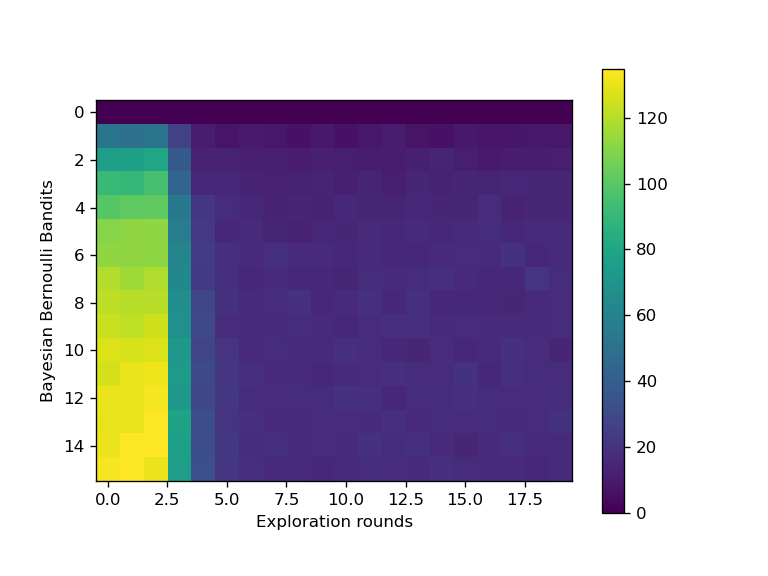
\includegraphics[height=1.1\textheight]{Figure 7.png}
    \end{center}
  \end{frame}
  \begin{frame}[t]
    \frametitle{Motivation}
    \framesubtitle{Goals}
    \begin{itemize}
      \item Identify the "Best" treatment : \textit{Exploration or Learning}
      \item Treat patients as "Effectively" as possible during the trial: 
      \textit{Exploitation or Earnings}
    \end{itemize}
  \end{frame}
  \begin{frame}[t]
    \frametitle{Introduction}
    \framesubtitle{Bayesian Bernoulli $K$-Armed Bandit Problem}
    Let $y_{k, t}\in \mathbf{Y}_{k, t}\sim \text{Ber}(\rho_{k})$, where:\\
    $\quad$Treatment $\equiv k\in\{1,\ldots, K\}\leftarrow$ Arm\\
    $\quad$Patient $\equiv t\in\{1,\ldots,N\}\leftarrow$ Time\\
    \color{white}.\color{black}\\
    The \textit{Bayesian} feature: $\rho_k \in \mathbf{P}_k\sim$ Beta($\alpha, \beta$)
    $ = \frac{\Gamma(\alpha + \beta)}{\Gamma(\alpha)\Gamma(\beta)}x^{\alpha - 1}
    x^{\beta - 1}$; \\
    $\quad$Conjugate Prior distribution\\
    \begin{equation*}
      (\alpha, \beta)=\left\{\begin{matrix}
        (S_{k, 0}, F_{k, 0})\in \mathbb{N}_+^2&\\
        (S_{k, 0} + S_{k, t}, F_{k, 0} + F_{k, t})&: t \geq 1
    \end{matrix}\right.
  \end{equation*}
  $\quad(\text{Succesful, Failure})\equiv(S_{k, t}, F_{k, t})\in\mathbb{N}_0^2$ 
  \end{frame}
  \begin{frame}[t]
    \frametitle{Introduction}
    \framesubtitle{Bayesian Bernoulli $K$-Armed Bandit Problem}
    \textit{Action} space:\\
    $\qquad\mathbb{A}_k \ni a_{k,t} = \{0 , 1\}$\\
    \color{white}.\color{black}\\
    Markovian \textit{transition probability rule}:\\
    $\qquad P_k\{\mathbf{s}_{k, t + 1} | \mathbf{s}_{k, t}, a_{k, t}\}\sim$
    \begin{equation*}
      \mathbf{s}_{k, t + 1} = \left\{\begin{matrix}
        \left\{\begin{array}{c}
          (S_{k, 0} + S_{k, t} + 1, F_{k, 0} + F_{k, t}): (S_{k, 0} + S_{k, t})/c_t\\
          (S_{k, 0} + S_{k, t}, F_{k, 0} + F_{k, t} + 1): (F_{k, 0} + F_{k, t})/c_t
        \end{array}\right.&:a_{k,t} = 1\\
        \mathbf{s}_{k, t} &: a_{k, t} = 0
      \end{matrix}\right.
    \end{equation*}
    \begin{equation*}
      \qquad c_t = S_{k, 0} + S_{k, t} + F_{k, 0} + F_{k, t}
    \end{equation*}
    \begin{equation*}
      R(\mathbf{s}_{k, t}, a_{k, t}) = \frac{S_{k, 0} + S_{k, t}}{c_t}a_{k, t}
    \end{equation*}
  \end{frame}
  \begin{frame}[t]
    \frametitle{Introduction}
    \framesubtitle{Objective}
    \begin{equation*}
      V^*_\pi(\mathbf{s}) = \max_\pi\mathbb{E}_\pi\left[\sum_{t = 1}^N\gamma^t
      \sum_{k = 1}^KR(\mathbf{s}_{k,t}, a_{k,t})|\mathbf{s}_0 = \mathbf{s}\right]
    \end{equation*}
    Bayesian regret
    \begin{equation*}
      R_{-1} = N\max_k(\rho_k) - \mathbb{E}_\pi\left[\sum_{k = 0}^K\sum_{t = 1}^Na_{k,t}y_{k,text}\right]
    \end{equation*}
  \end{frame}
  \begin{frame}
    \begin{center}
      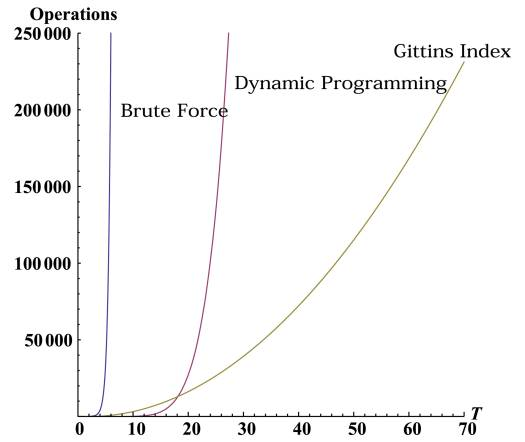
\includegraphics[height=\textheight]{DP.jpeg}
    \end{center}
  \end{frame}
\end{document}